%!TEX program = xelatex
\documentclass[xcolor={table}]{beamer}

\usepackage[brazil]{babel}	
\usepackage[utf8]{inputenc}
\usepackage[T1]{fontenc}
\usepackage[scaled]{helvet}
\usepackage{amsthm}
\usepackage{ragged2e}
\usepackage{subfig}
\usepackage[table]{xcolor}
\usepackage{multicol}
\usepackage{multirow}
\usepackage{fancyvrb}
\usepackage{verbatim}
\usepackage{hyperref}

\usetheme{Execushares}

\title{Laborator 2 - UART}
\subtitle{}
\author{Coca Mihai \\
        Ioana Dragoș}

\setcounter{showSlideNumbers}{1}

\begin{document}
	\setcounter{showProgressBar}{0}
	\setcounter{showSlideNumbers}{0}

	\frame{\titlepage}

	\begin{frame}
		\frametitle{Tabelă de Conținut}
		\begin{enumerate}
			\item Serial vs Paralel
            \item Concepte teoretice
			\item Configurare
			\item Exemplu practic
		\end{enumerate}
	\end{frame}

	\setcounter{framenumber}{0}
	\setcounter{showProgressBar}{1}
	\setcounter{showSlideNumbers}{1}
	
	\section{Serial vs Paralel}
	\begin{frame}
	    \frametitle{Comunicație paralelă}
	    \begin{itemize}
	        \item \textbf{\textit{Comunicația paralelă}} - metodă de a transmite mai multe valori binare simultan
	    \end{itemize}
	    \begin{figure}
	        \centering
	        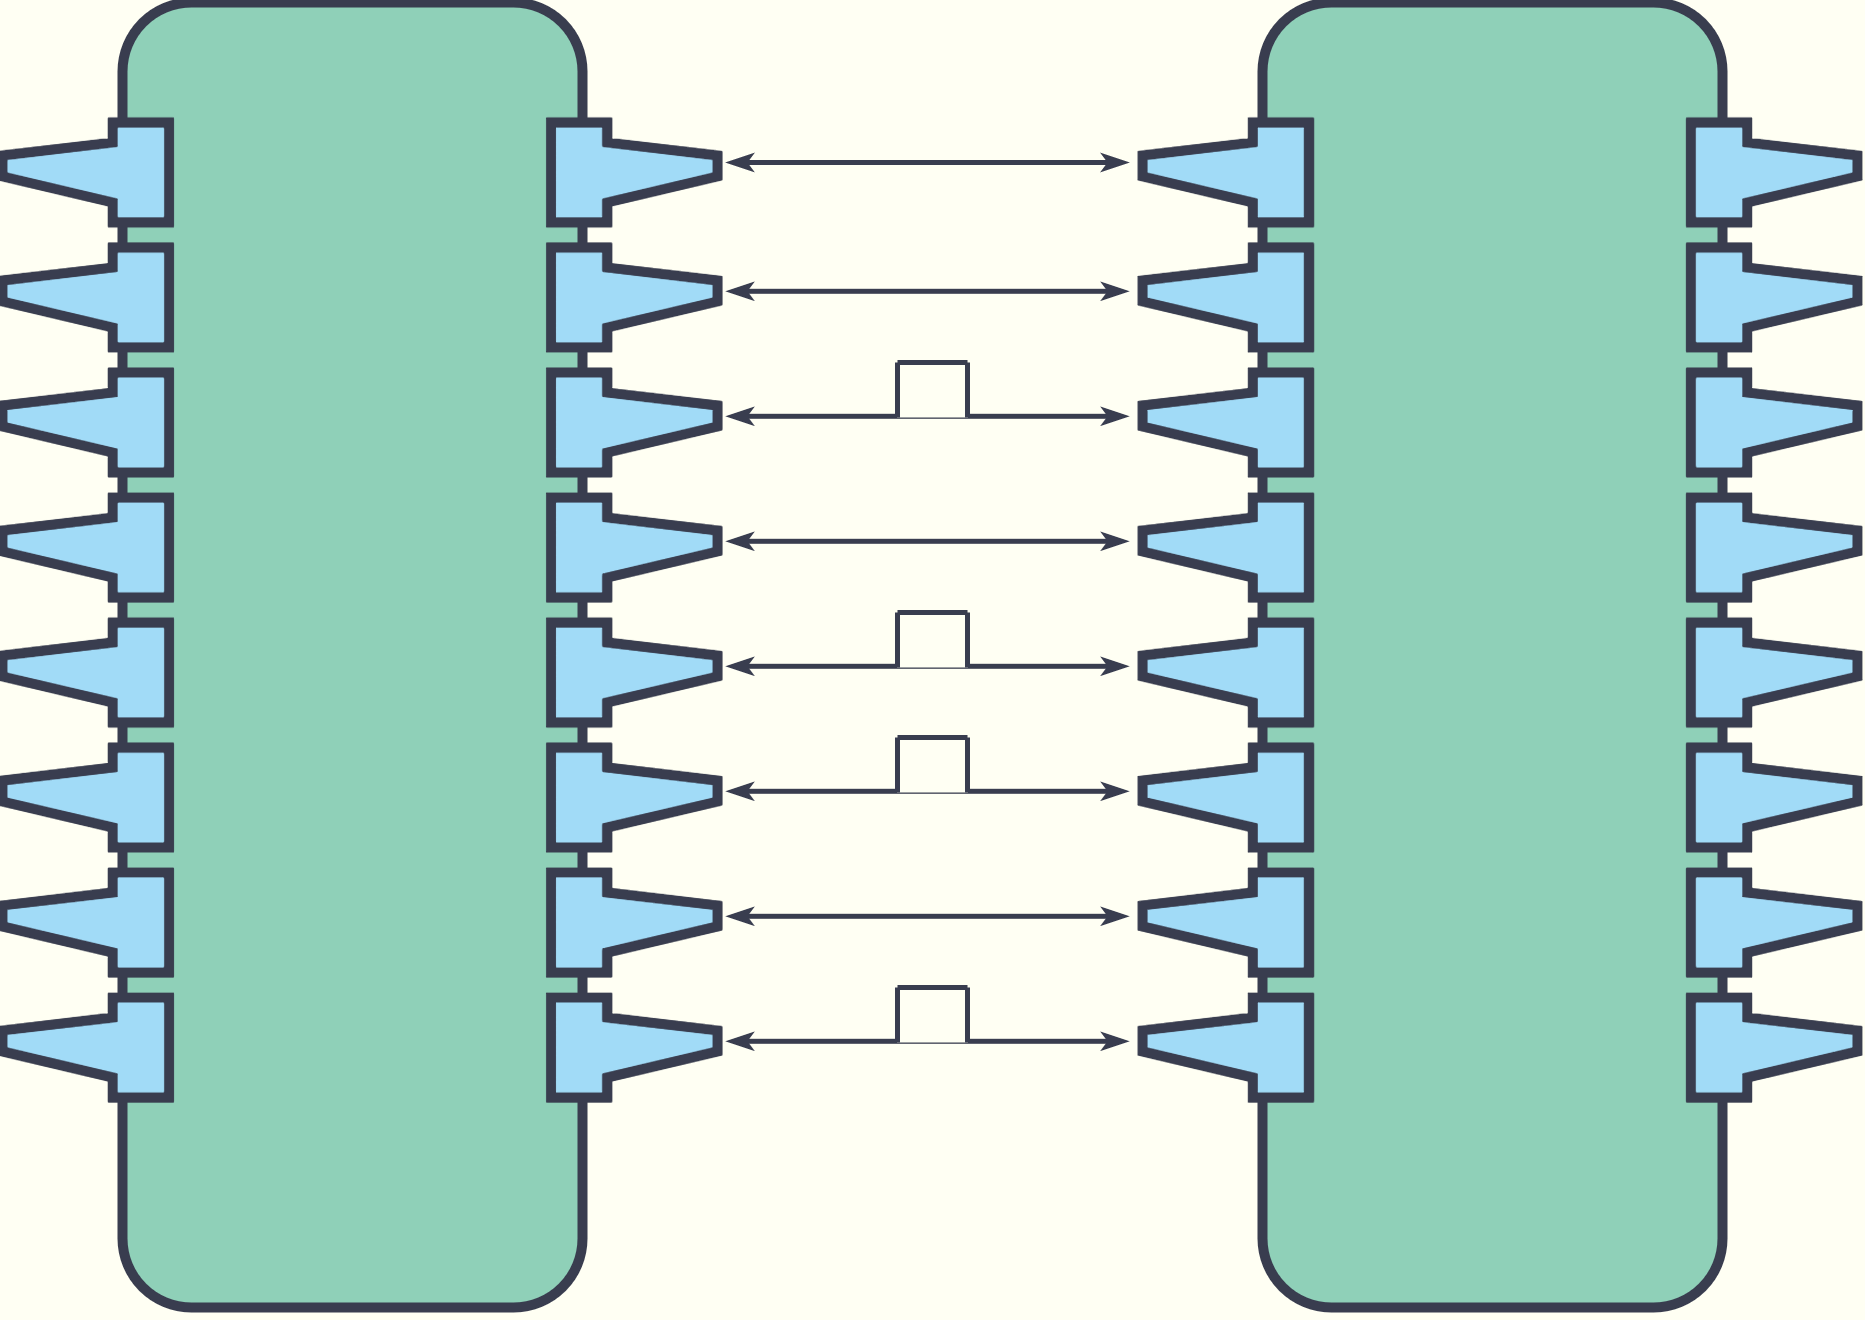
\includegraphics[width=6.5cm]{images/paralel1.png}
	        \caption{Exemplu de comunicație paralelă}
	        \label{fig:my_label}
	    \end{figure}
	\end{frame}
	\begin{frame}
	    \frametitle{Comunicație serială}
	    \begin{itemize}
	        \item \textbf{\textit{Comunicația serială}} - metodă de a transmite câte un bit la un moment de timp
	        \begin{itemize}
	            \item \textbf{\textit{Avantaj}} - costul mai mic de implementare, fiind nevoie de 1 fir pentru o comunicație unidirecțională \textbf{\textit{half-duplex}}, respectiv 2 fire pentru \textbf{\textit{full-duplex}}
	            \item \textbf{\textit{Dezavantaj}} - durată mai mare de transmisie a datelor
	        \end{itemize}
	    \end{itemize}
	    \begin{figure}
	        \centering
	        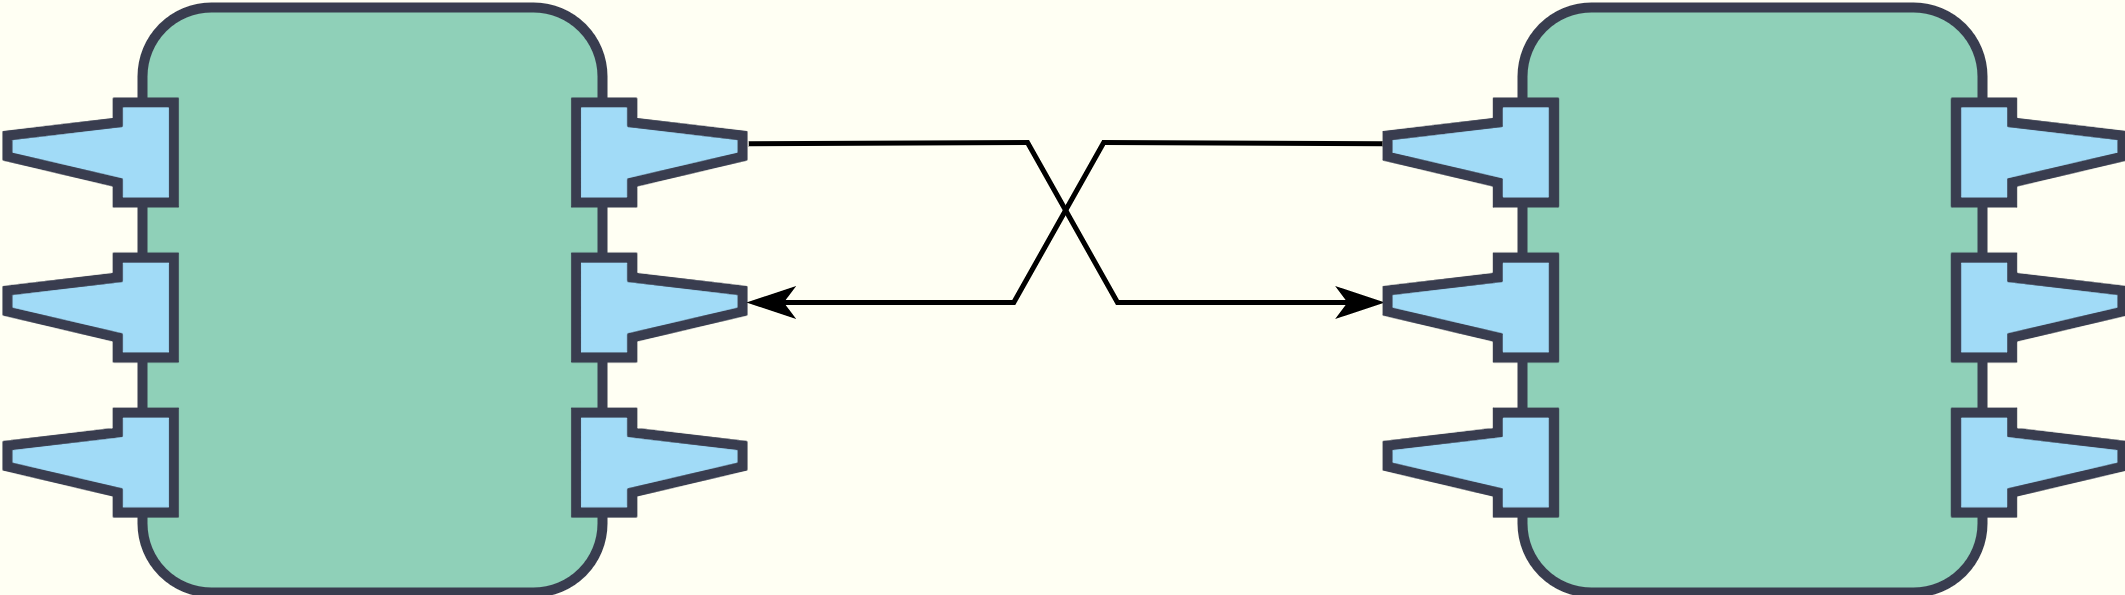
\includegraphics[width=7cm]{images/serial1.png}
	        \caption{Exemplu de comunicație serială}
	        \label{fig:my_label}
	    \end{figure}
	\end{frame}
	\section{Concepte teoretice}
	\begin{frame}
		\frametitle{UART}
		\begin{itemize}
		    \item \textbf{\textit{Universal Asynchronous Receiver/Transmitter}}
		    \item \textbf{\textit{UART}} - protocol de comunicație care se folosește de comunicația serială asincronă și rata(viteza) configurabilă de transmisie \\
		    \textbf{\textit{Baud Rate - biți/s}}
		    \item Sistemele embedded, microcontroller-ele folosesc preponderent \textbf{\textit{UART}} ca și protocol de comunicație între dispozitive, datorită facilității de configurare, cât și a faptului că sunt folosite doar două semnale
		    \begin{itemize}
		        \item \textbf{\textit{RX}} - Recepție
		        \item \textbf{\textit{TX}} - Transmisie
		    \end{itemize}
		\end{itemize}
	\end{frame}
		\begin{frame}
		\frametitle{Transmisia datelor}
		\begin{itemize}
		    \item Datele sunt transmise sub formă de cadre, de lungime configurabilă, alcătuite din : \\
		    \begin{figure}
		        \centering
		        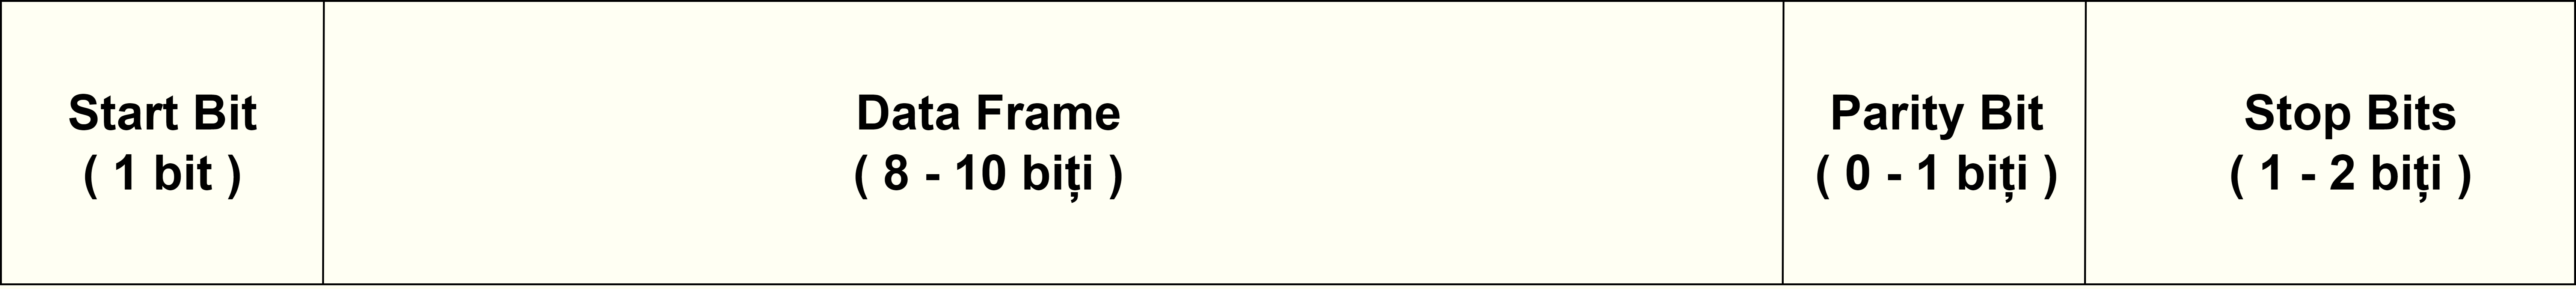
\includegraphics[width=7cm]{images/cadru.png}
		    \end{figure}
		    \begin{itemize}
		        \item \textbf{\textit{Start Bit}} - întrucât linia de transmisie este ținută la nivelul logic 1 atunci când este inactivă, pentru a începe transferul, se realizează o tranziție \textbf{$ 1 \rightarrow 0$}, moment în care dispozitivul care recepționeză va citi biți la frecvența setată prin \textbf{\textit{baud rate}}
		        \item \textbf{\textit{Data Frame}} - 8/9/10 biți de date propriu-zise
		        \item \textbf{\textit{Parity Bit}} - formă de verificare a integrității datelor la nivel de 1 bit
		        \item \textbf{\textit{Stop Bits}} - 1/2 biți folosiți pentru a semnala sfârșitul pachetului, reprezentați printr-o tranziție \textbf{$0 \rightarrow 1 $}
		    \end{itemize}
		\end{itemize}
		\end{frame}
		\begin{frame}
		    \frametitle{Pașii unei transmisiuni}
		    \begin{enumerate}
		        \item Dispozitivul UART care transmite primește datele în paralel de la magistrala de date
		        \item Dispozitivul UART care transmite adaugă biții de start, paritate și stop la cadrul de date
		        \item Întregul pachet este transmis serial către dispozitivul UART care recepționeză, care va eșantiona semnalul primit în funcție de baud rate-ul preconfigurat înaintea începerii comunicației
		        \item Dispozitivul UART care recepționează va înlătura biții de start, paritate și stop și va transfera paralel datele către magistrală
		    \end{enumerate}
		\end{frame}
        \section{Configurare}
        \begin{frame}
                \frametitle{ \href{https://github.com/undacmic/MCULabs/blob/main/Resurse/FRDM-KL25Z_ReferenceManual.pdf}{Setarea regiștrilor}}
                \begin{itemize}
                    \item Activarea semnalului de ceas pentru a putea configura modulele folosite 
                    \begin{itemize}
                        \item \textbf{\textit{SIM\_SCGC4}} - modul periferic UART
                        \item \textbf{\textit{SIM\_SCGC5}} - portul de pe care vom folosi pinii pentru recepție și transmisie
                    \end{itemize}
                    \item \textbf{\textit{UARTx\_C2 - biții RE/TE }} - activarea/dezactivarea bitului de emițător/receptor pentru a putea configura modulul
                    \item \textbf{\textit{UARTx\_C1 - biții M/PE/PT}} - setarea numărului de biți de date propriu-zise și configurarea parității
                    \item \textbf{\textit{UARTx\_BDH}} și \textbf{\textit{UARTx\_BDL}} - setarea baud rate-ului
                    \item \textbf{\textit{UARTx\_C4\_OSR}} - setarea ratei de eșantionare per bit-time
                    \item \textbf{\textit{PORTx\_PCR}} - multiplexarea semnalului pe pini
                \end{itemize}
        \end{frame}
        \section{Exemplu practic}
        \begin{frame}
                \frametitle{Experiment}
                \begin{itemize}
                    \item Urmăriți pașii din laborator pentru a configura corect modulul periferic UART
                    \item Instalarea aplicației \href{https://wiki.mta.ro/_media/c/4/ssmp/environment_setup.7z}{\textbf{\textit{PuTTY}}} prezentă în arhiva de materiale a laboratorului
                    \item Stabilirea unui baud rate, care va fi folosit atât de codul încărcat pe platforma de dezvoltare, cât și de către terminalul ce urmează a fi deschis
                    \item Conectarea plăcuței prin USB la calculator va determina apariția unei noi intrări în $\textit{\textbf{Device Manager}} \rightarrow \textbf{\textit{Ports (COM \& LPT)}}$
                \end{itemize}
        \end{frame}
        \begin{frame}
                \frametitle{Experiment}
                \begin{figure}
                    \centering
                    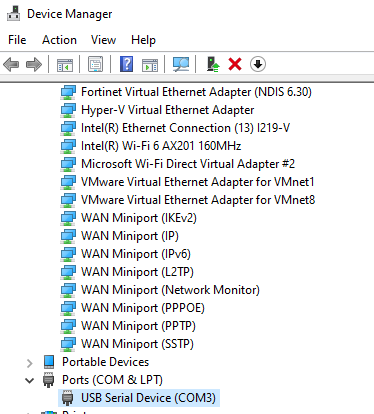
\includegraphics[width=5cm]{images/device.png}
                    \label{ceva}
                    \caption{ Identificarea portului pe care se află plăcuța}
                \end{figure}
        \end{frame}
        \begin{frame}
                \frametitle{Experiment}
                \begin{figure}
                    \centering
                    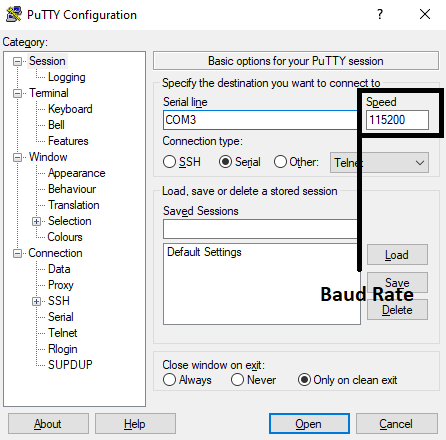
\includegraphics[width=6cm]{images/putty1.png}
                    \caption{Configurarea terminalului}
                \end{figure}
        \end{frame}
        \begin{frame}
                \frametitle{Experiment}
                \begin{itemize}
                    \item Vom transmite prin UART caracterul \\ 
                    \textbf{\textit{o}} - \textbf{\textit{0x6F}} - \textit{\textbf{0110 1111}}
                    \item Pentru vizualizare vom utiliza osciloscopul digital \textbf{\textit{Analog Discovery}} prin intermediul aplicației \textit{Waveforms} pe care vom configura canalul 1 cu baud rate-ul setat pe plăcuță
                    \begin{itemize}
                        \item \textbf{\textit{1+}} - conectat cu pinul de TX (\textbf{\textit{PTA2}})
                        \item \textbf{\textit{1-}} - conectat la GND al plăcuței pentru a avea aceeși tensiune de referință
                    \end{itemize}
                \end{itemize}
        \end{frame}
        \begin{frame}
                \frametitle{Rezultat}
                \begin{figure}
                    \centering
                    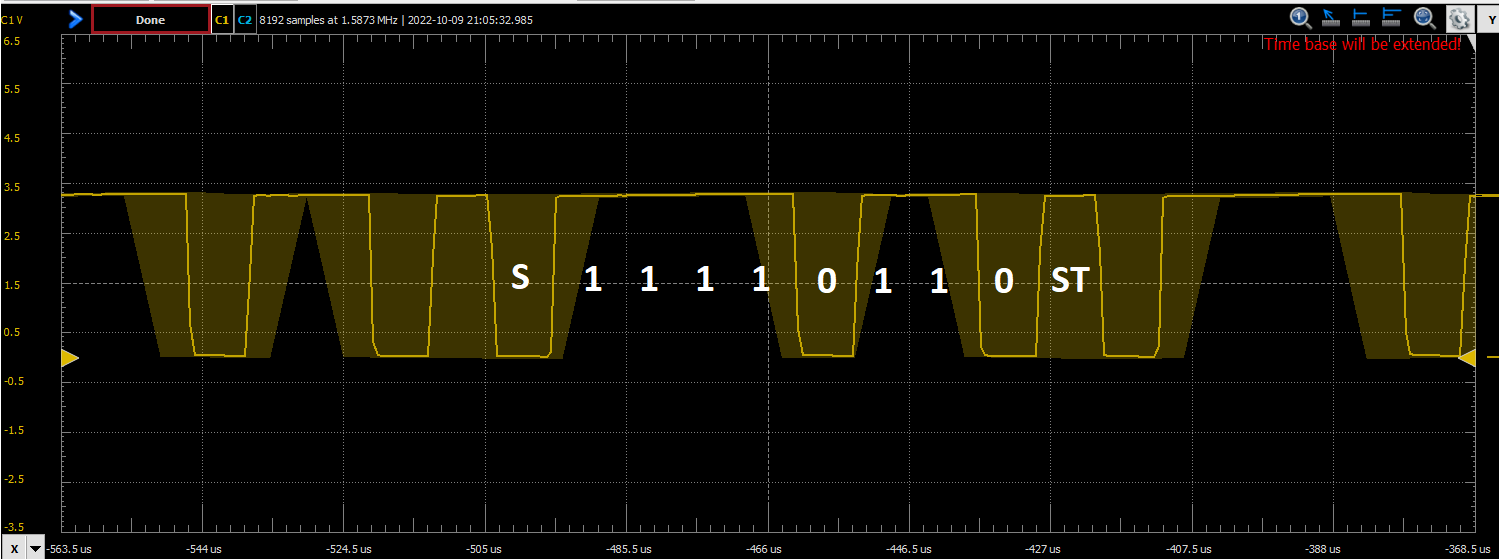
\includegraphics[width=11cm]{images/osciloscop.png}
                    \caption{Semnalul obținut de osciloscop}
                    \label{fig:my_label}
                \end{figure}
        \end{frame}
	\appendix


\end{document}